\documentclass[compress]{beamer} %compress f�r komprimierte Darstellung der Navigationsleiste


\usepackage[ngerman]{babel}   % W�hlt die Sprache
\usepackage{graphicx}          % Einf�gen von Grafiken
\usepackage[T1]{fontenc}     	% Bestimmt das Encoding der Schriften
\usepackage[latin1]{inputenc} % Bestimmt das Encoding der Datei. 
\usepackage{pgf,pgfarrows}		% pgfnodes,pgfautomata,pgfheaps,pgfshade

\usetheme{Warsaw}

% Use some nice templates
\beamertemplatetransparentcovereddynamic	% verdeckte Slides transparent anzeigen
\beamertemplatenavigationsymbolsempty			% Navigationssymbole ausblenden


\title[CYBOP]{
  Untersuchung der Realisierungsm�glichkeiten von CYBOL -
  Webfrontends, unter Verwendung von Konzepten des Cybernetics
  Oriented Programming (CYBOP)}
\author{Rolf Holzm�ller}
\institute{
  Fachgebiet Softwaresysteme/Prozessinformatik
}
\date{
  Diplomverteidigung\\
  11. Juli 2005}
  

\begin{document}


  %footline mit Seitennummerierung
%	\setbeamertemplate{footline}
%	{%
%	  \leavevmode%
%	  \hbox{\begin{beamercolorbox}[wd=.5\paperwidth,ht=2.5ex,dp=1.125ex,leftskip=.3cm plus1fill,rightskip=.3cm]
%	          {author in head/foot}%
%	          \usebeamerfont{author in head/foot}\insertshortauthor
%	        \end{beamercolorbox}%
%	        \begin{beamercolorbox}[wd=.25\paperwidth,ht=2.5ex,dp=1.125ex,leftskip=.3cm,rightskip=.3cm plus1fil]
%	          {title in head/foot}%
%	          \usebeamerfont{title in head/foot}\insertshorttitle
%	        \end{beamercolorbox}%
%	        \begin{beamercolorbox}[wd=.25\paperwidth,ht=2.5ex,dp=1.125ex,leftskip=.3cm plus1fill,rightskip=.3cm]
%	          {title in head/foot}%
%	          \usebeamerfont{title in head/foot}\insertframenumber/\inserttotalframenumber
%	        \end{beamercolorbox}
%	  }%
%    \vskip0pt%
%  }


  %Titelfolie
  \begin{frame}
   
    \titlepage
    
  \end{frame}


  %Gliederung
  \begin{frame}

    \frametitle{Gliederung}
    \tableofcontents

  \end{frame}
  
  %Folien vor jeden Kapitel
  \AtBeginSection[]
  {

    \begin{frame}
      \frametitle{Gliederung}
      \tableofcontents[current]
    \end{frame}

  }
  
  %Einleitung  
  \section{Einleitung}
  
  \begin{frame}

     \frametitle{Einleitung}
     
     \begin{block}<1->{Aufgabe}
       \begin{itemize}
         %\item Untersuchen von Realiserungsm�glichkeiten in CYBOP f�r
         %      die Darstellung in Webfrontends
         \item Erweiterung des Beschreibungssprache CYBOL f�r Webanwendungen
         \item Erweiterung des Interpreters CYBOI f�r Webanwendungen
         \item Integration eines Webservers in CYBOI
         \item Entwicklung eines Prototypen zur Veranschaulichung der Realisierbarkeit
       \end{itemize}
     \end{block}

     \begin{block}<2->{Abgrenzung}
       Es war nicht das Ziel dieser Arbeit, die Sinnhaftigkeit 
       des CYBOP Ansatzes zu begr�nden.
     \end{block}
     
  \end{frame}

  \section[CYBOP]{Cybernetics Oriented Programming (CYBOP)}
  \begin{frame}
    \frametitle{CYBOP}
  
    \begin{block}<1->{Definition}
      Fundamental principles of human thinking are Discrimination, 
      Categorization and Composition. The abstractions they deliver are 
      Item, Category and Compound.
    \end{block}
    
    \begin{block}<2->{Prizipien von CYBOP}
    
      \begin{itemize}
        
        \item<2-2> Discrimimation
        \item<3-3> Categorization
        \item<4-4> Composition
      
      \end{itemize}
    
    \end{block}
    
  \end{frame}


  \section[CYBOL]{Cybernetics Oriented Language (CYBOL)}
  \subsection{Sprachelemente}
  \begin{frame}

    \frametitle{Sprachelemente}
    
    \begin{block}<1->{Allgemeines}
      \begin{itemize}
        \item XML-Syntax
        \item einheitliche Beschreibung f�r alle Sachverhalte
      \end{itemize}
    \end{block}

    \begin{columns}

      \column{5cm}
        \begin{block}<2->{Elemente}
          \begin{center}
            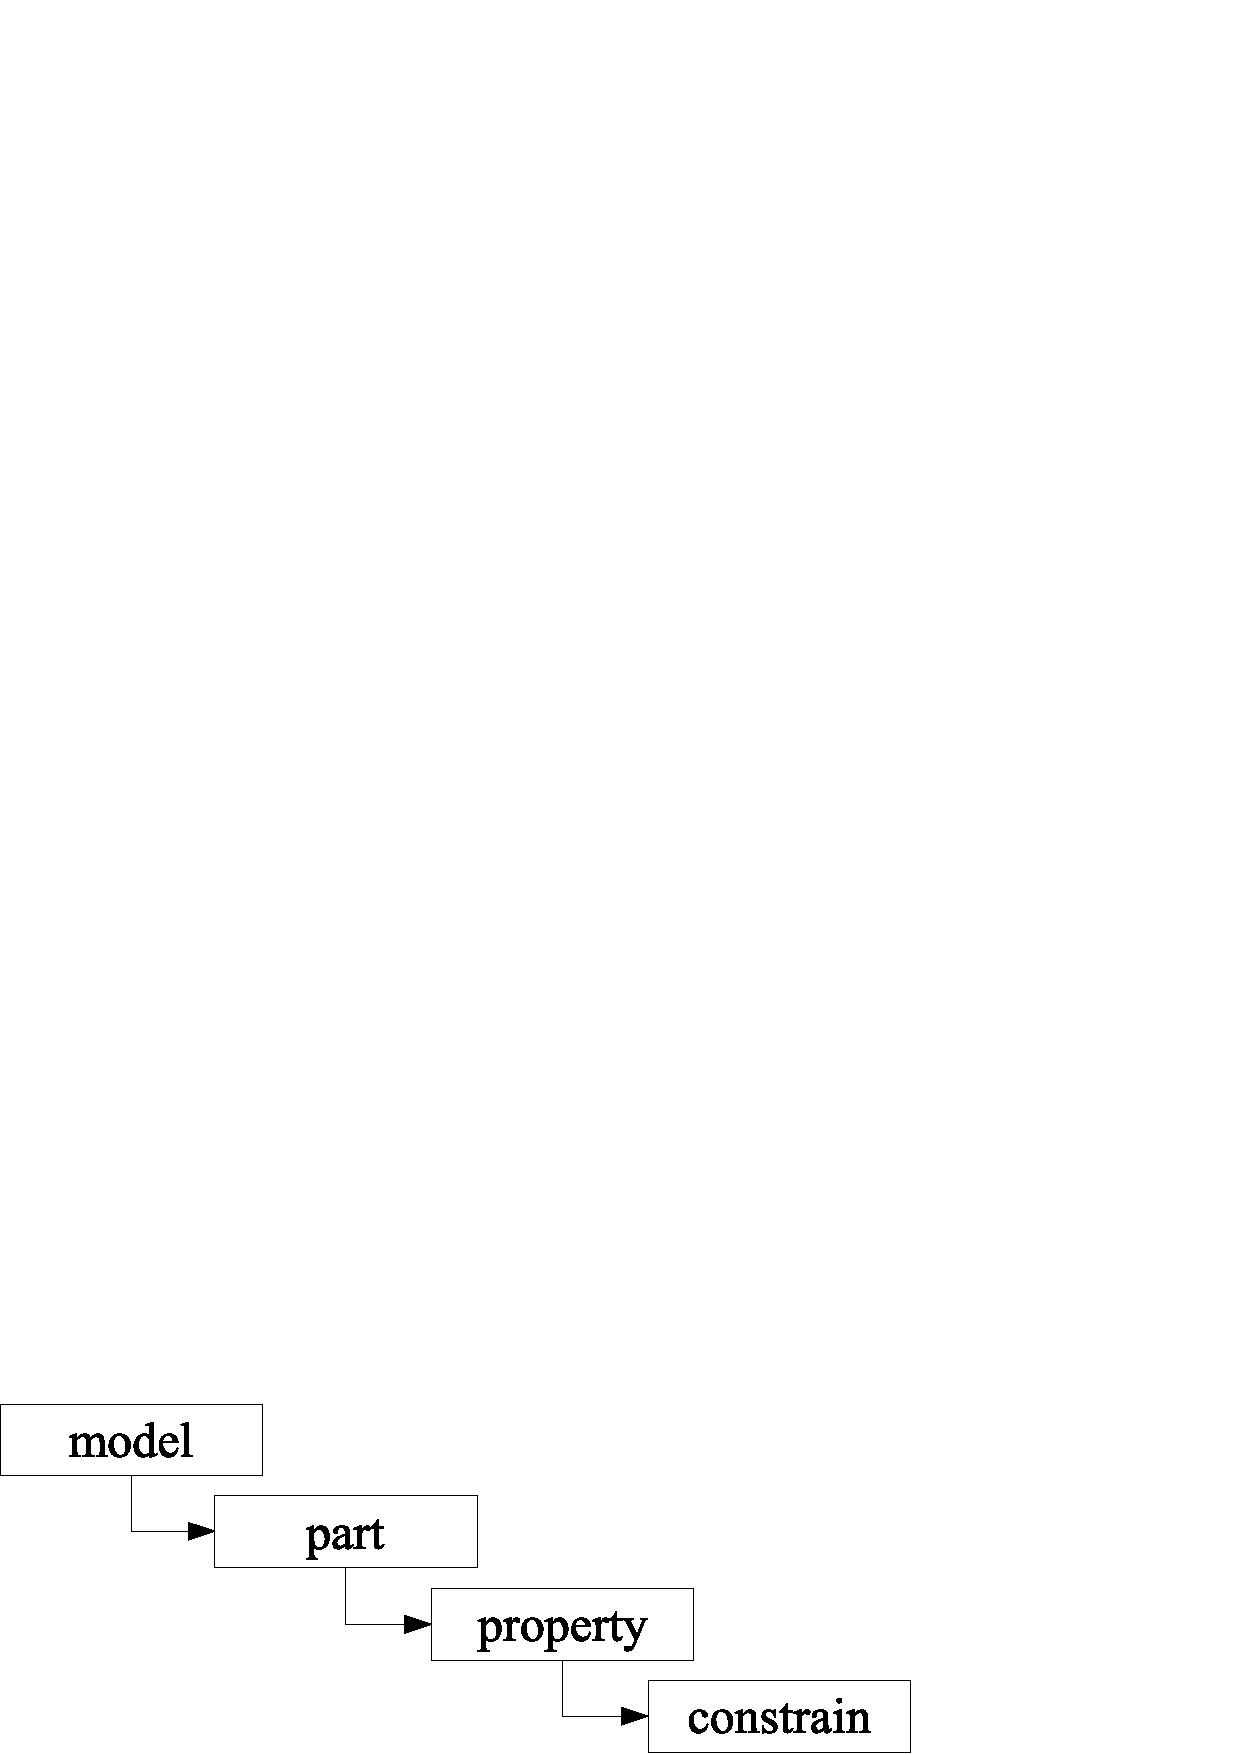
\includegraphics[height=1.92cm]{images/elementecybol.pdf}
          \end{center}      
        \end{block}
    
      \column{5cm}
        \begin{block}<2->{Attribute der Elemente}
          \begin{itemize}
            \item name
            \item channel
            \item abstraction
            \item model
          \end{itemize}
        \end{block}

    \end{columns}

  \end{frame}
  
  \subsection[Beschreibungs.]{Beschreibungsm�glichkeiten f�r Webfrontends}
  \begin{frame}
  
    \frametitle{Beschreibungsm�glichkeiten f�r Webfrontends}
  
    \begin{block}<1->{Beschreibungsm�glichkeiten}
    
      \begin{itemize}
        \item Clientseitige Beschreibungssprachen (HTML, XHTML)
        \item Clientseitige Skriptsprachen (Javascript)
        \item Serverseitige Skript-/Programmiersprachen \\(PHP, JSP, ASP, ...)
      \end{itemize}
      
    \end{block}
    
    \begin{block}<2->{Auswahl}
    
      \LARGE{ $\Rightarrow$ XHTML }
    \end{block}
      
    \begin{block}<3->{Erweiterung f�r Webfrontends}
    
      \begin{itemize}
        \item Keine Syntaktischen �nderungen von CYBOL
        \item Zwei neue Properties (html\_tag, html\_tag\_properties)
      \end{itemize}
      
    \end{block}
    

  \end{frame}
  

  \subsection{Beispiel}
  \begin{frame}[fragile]
    \frametitle{Beispiel}
    
    \begin{block}{Beipspiel in CYBOL}
      \small{
\begin{verbatim}
<model>
  <part name="edit_button" channel="inline" 
        abstraction="string" model="edit">
    <property name="html_tag" channel="inline" 
              abstraction="string" model="a"/>
    <property name="html_tag_properties" channel="inline" 
              abstraction="string" 
              model="href='edit.cybol'"/>
  </part>
</model>
\end{verbatim}
      }
    \end{block}
    
    \begin{block}{generiertes XHTML}
      \small{
\begin{verbatim}
<a href='edit.cybol'>
   edit
</a>
\end{verbatim}
      }
    \end{block}
    
\end{frame}

  \section[CYBOI]{Cybernetics Oriented Interpreter (CYBOI)}
  \subsection{Signal Memory}
  \begin{frame}
    \frametitle{Signal Memory}

    \begin{columns}

      \column{5cm}
        \begin{block}<1->{Signal Memory}
    
          \begin{itemize}
            \item Zentrale Struktur f�r Speicherung von Signalen in CYBOP
            \item Signalwarteschleife
            \item Abarbeitung in Endlosschleife
          \end{itemize}
    
        \end{block}

    \column{5cm}
      \begin{block}<2->{Signalabarbeitung}
      
        \begin{center}
          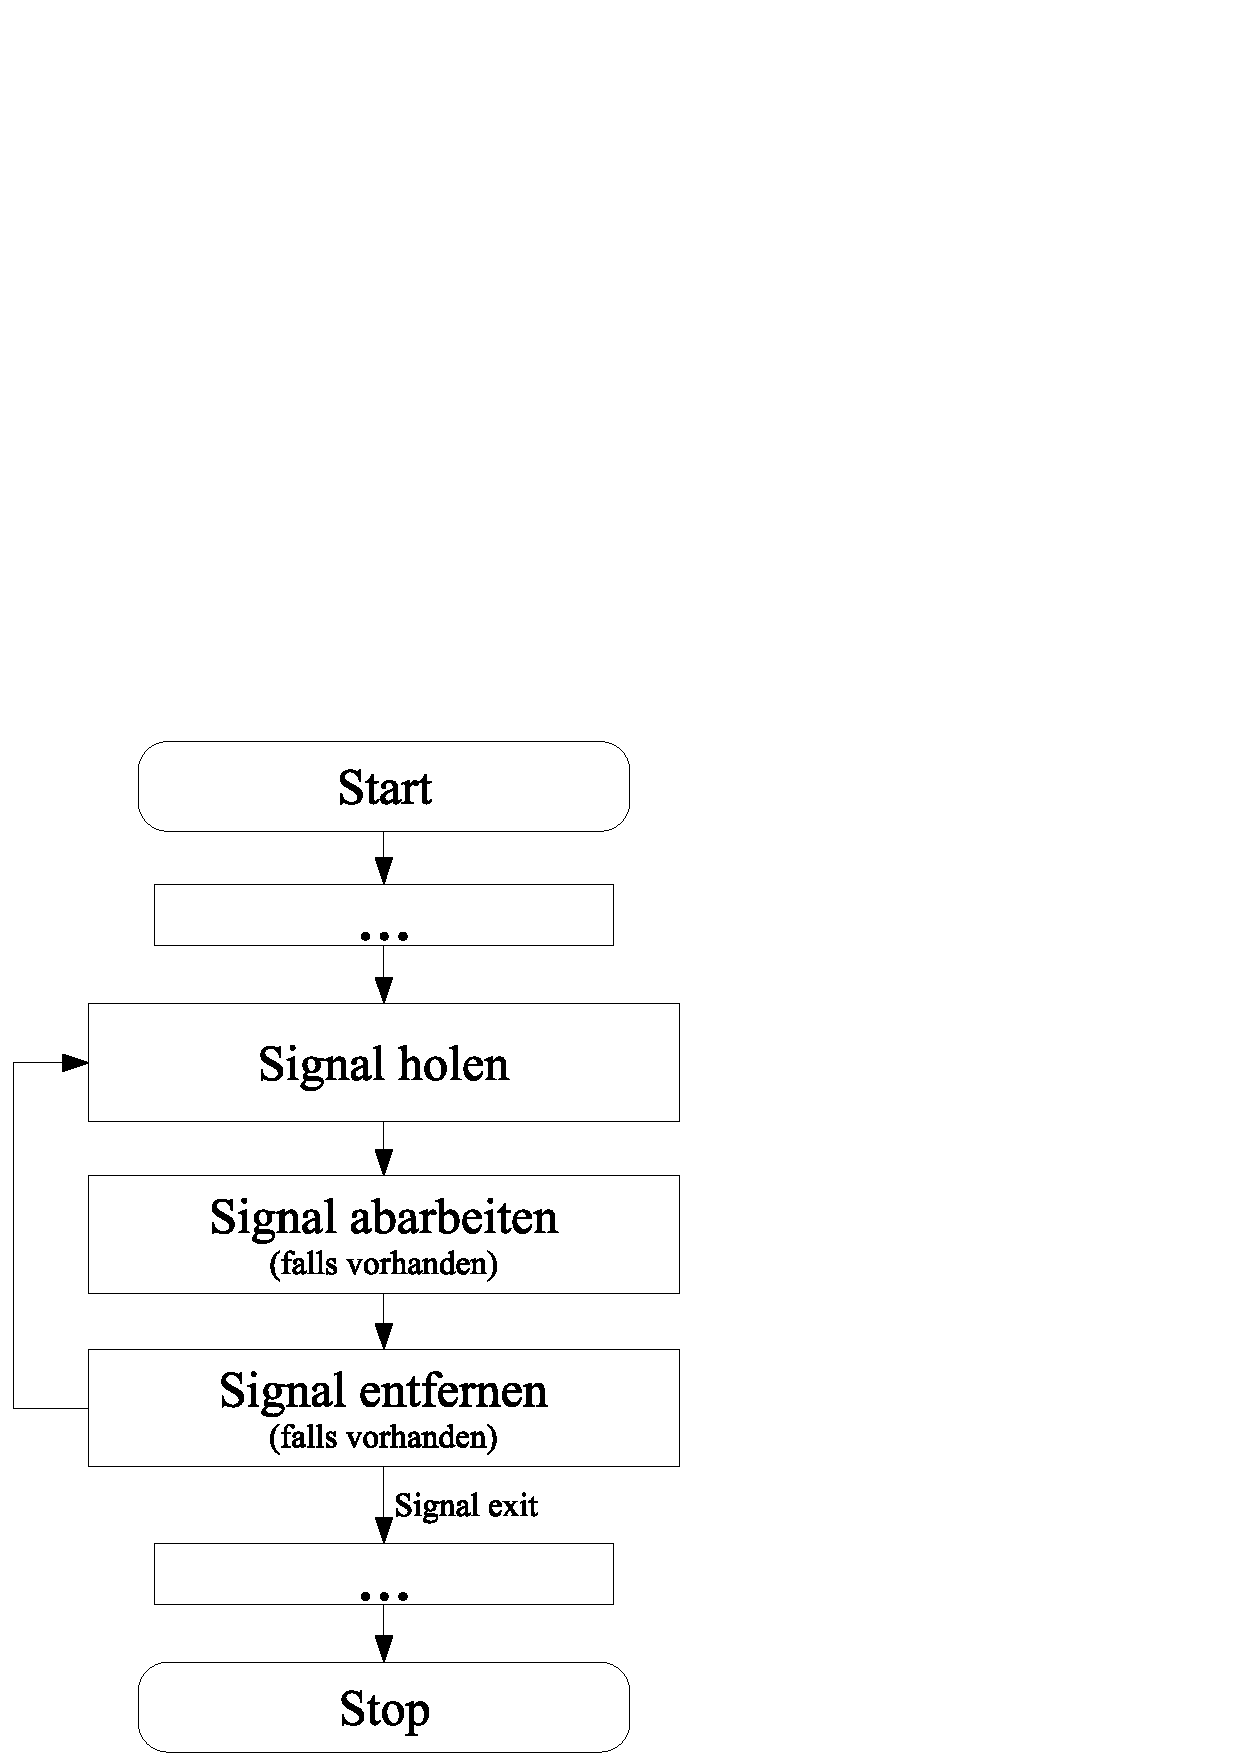
\includegraphics[height=6cm]{images/signalabarbeitung.pdf}
        \end{center}

      \end{block}
    \end{columns}    
  
  \end{frame}


  \subsection{Knowledge Memory}
  \begin{frame}
    \frametitle{Knowledge Memory (1)}

    \begin{columns}
    
        
      \column{5cm}
        \begin{block}{Knowledge Memory}
        
          \begin{itemize}
          
            \item Zentrale Struktur f�r alles Wissen
            \item Hierarchisch aufgebaut
            \item durch Compound realisiert
          \end{itemize}
        \end{block}

      \column{5cm}
        \begin{block}{Knowledge Memory}
          \begin{center}
          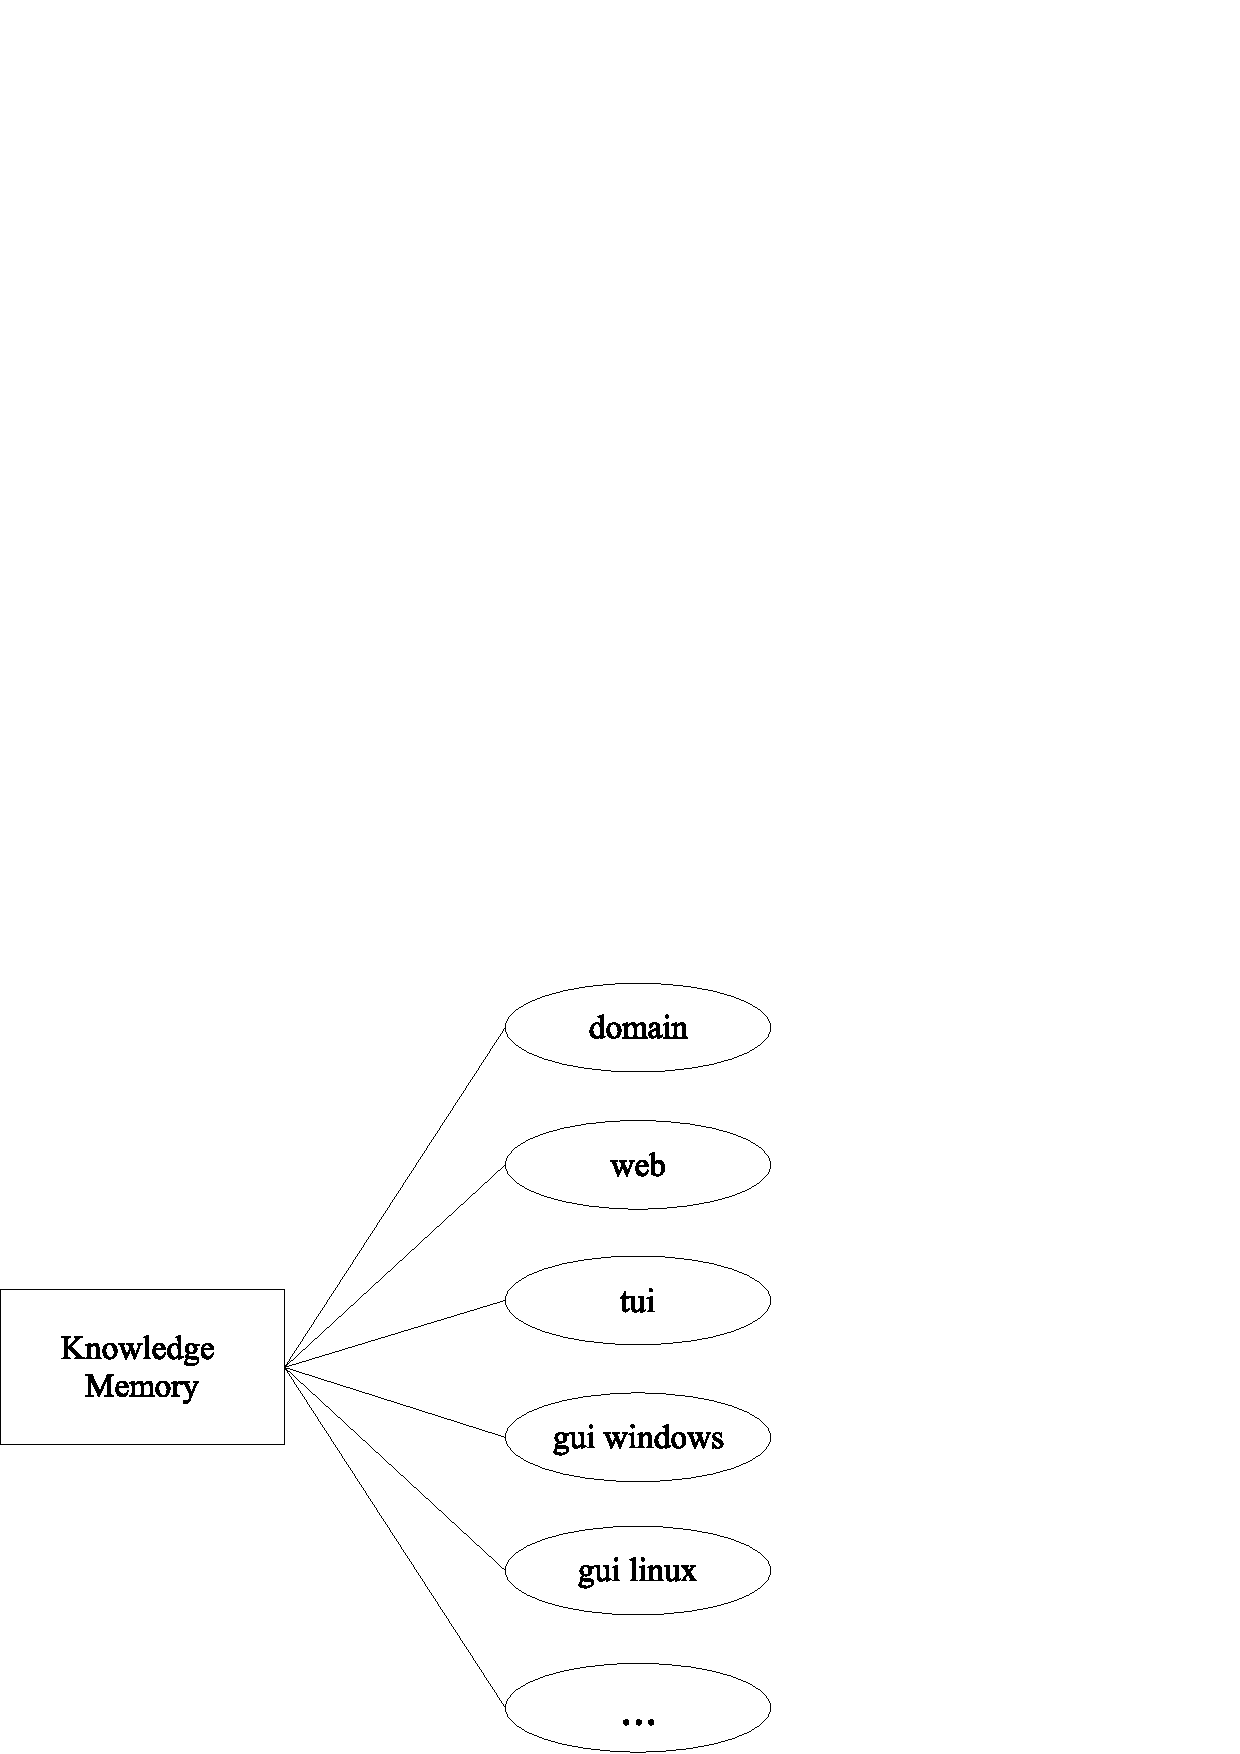
\includegraphics[height=6cm]{images/knowledgememory.pdf}
          \end{center}
        \end{block}
    \end{columns}
  
  \end{frame}
  
  \begin{frame}
    \frametitle{Knowledge Memory (2)}

    \begin{block}{Bsp. Abbildung des Knowledge Memory}

      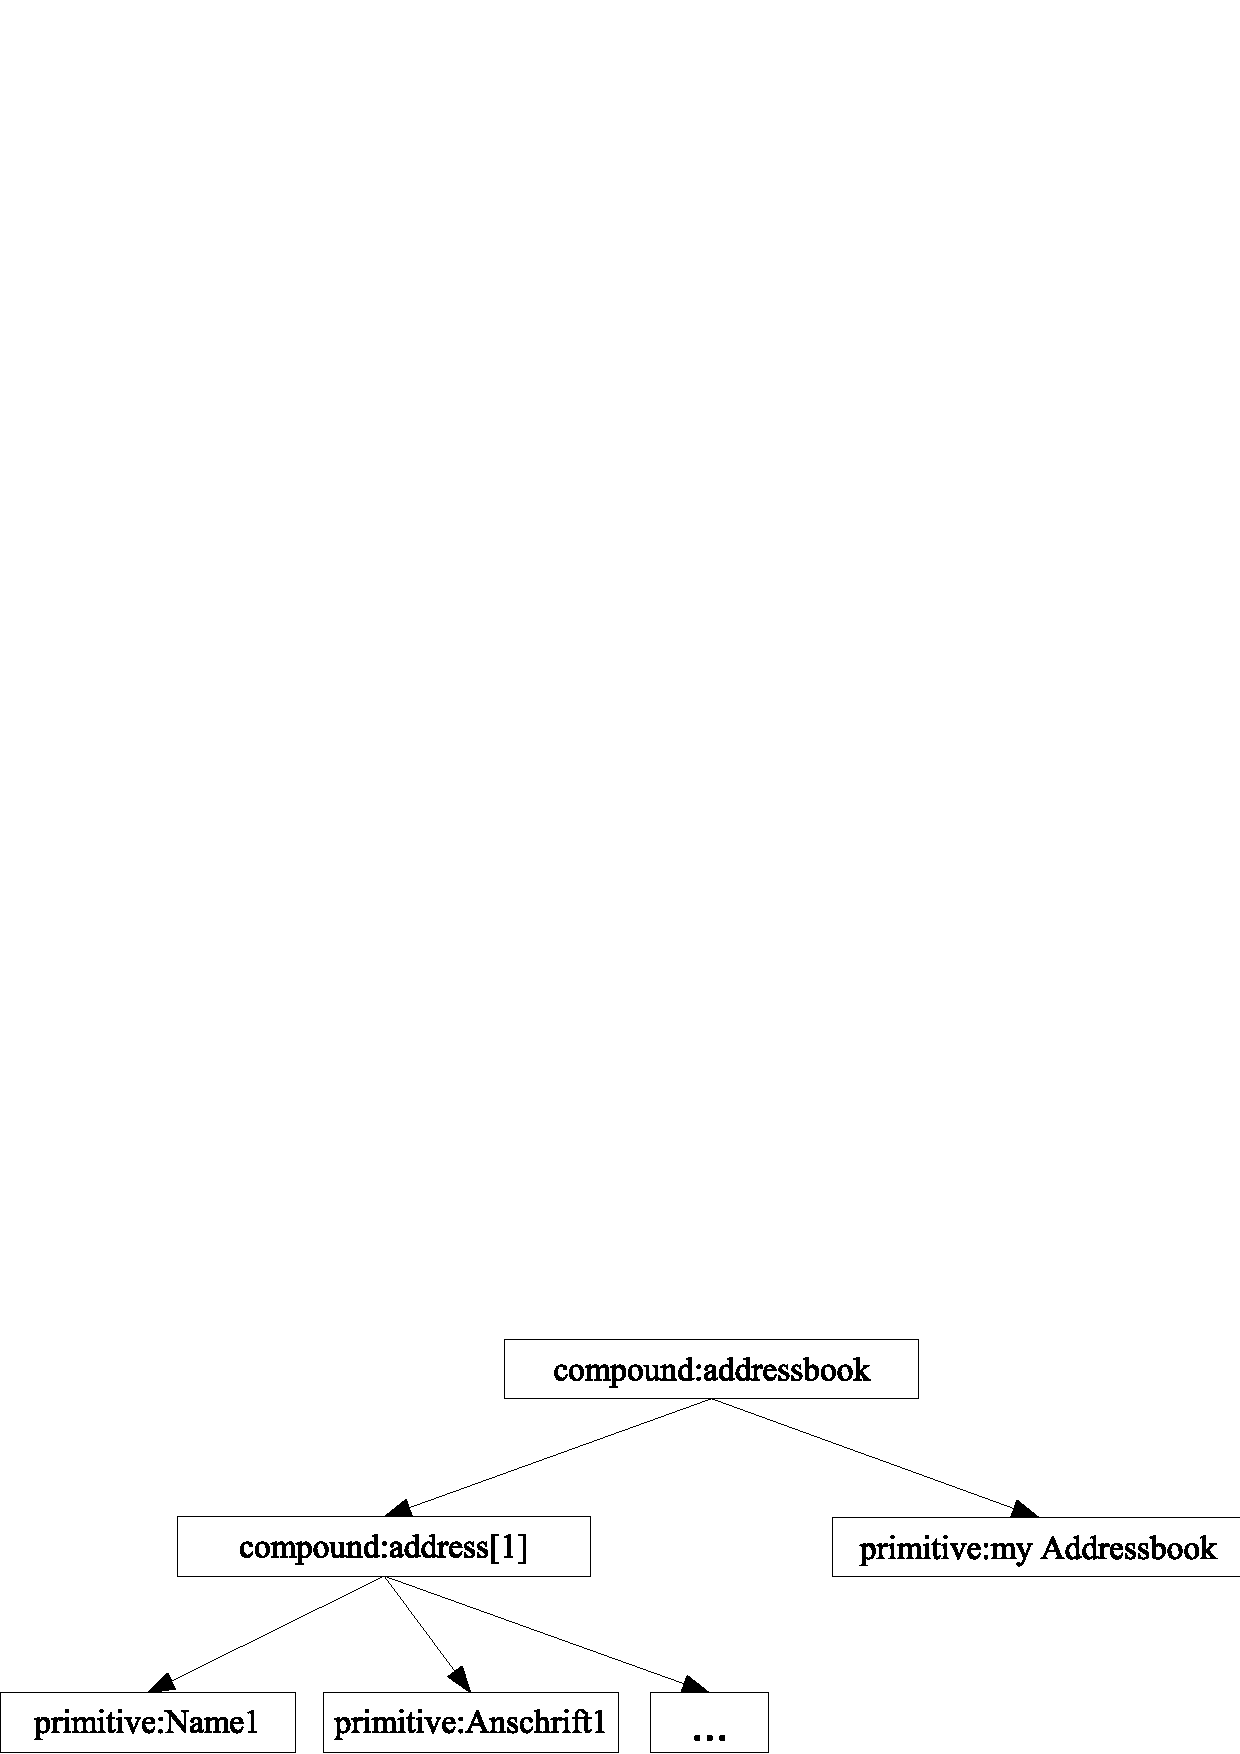
\includegraphics[width=10cm]{images/compositum.pdf}
    
    \end{block}
  
  \end{frame}
  
  \subsection[Integration]{Integration des Webservers}

  \begin{frame}
    \frametitle{Integration des Webservers}

    \begin{block}<1->{Vorgedanken}

      \begin{itemize}
        \item<1-> \textbf<2->{blockierende} vs. nichtblockierende \textbf<2->{Sockets}
        \item<2-> $\rightarrow$ Thread
        \item<3-> $\rightarrow$ Synchronisation
      \end{itemize}
    
    \end{block}

    \begin{block}<4->{Architektur}

      \includegraphics[width=10cm]{images/integration.pdf}
    
    \end{block}
  
  \end{frame}

  \section[Zusammenfassung]{Zusammenfassung und Ausblick}
  \begin{frame}
    \frametitle{Zusammenfassung und Ausblick}
    
    \begin{block}<1->{Zusammenfassung}
      \begin{itemize}
        \item einfache Beschreibung
        \item CYBOL deckt Belange einer Webanwendung ab
        \item Integration eines Webservers in CYBOI
        \item funktionsf�higer Prototyp
      \end{itemize}
    \end{block}

    \begin{block}<2->{Ausblick}
      \begin{itemize}
        \item Abspeicherung des Wissens in Datenbank bzw. Dateien
        \item Editoren f�r Entwicklung
        \item Sessionverwaltung f�r Webserver
        \item Robustheit
      \end{itemize}
    \end{block}
  
  \end{frame}


  \begin{frame}
    \frametitle{Fragen?}
    
    \begin{block}
    
      \begin{center}
        Danke f�r Ihre Aufmerksamkeit.
      \end{center}
       
    \end{block}

    \begin{block}

      \begin{center}    
        Haben Sie noch Fragen? \\
        
        
\includegraphics[width=3cm]{images/melden3.pdf}

      \end{center}
    \end{block}
  \end{frame}
  

\end{document}

